% Chapter 1

\chapter{Introducción} % Main chapter title

\label{Chapter1} % For referencing the chapter elsewhere, use \ref{Chapter1} 

%----------------------------------------------------------------------------------------

% Define some commands to keep the formatting separated from the content 
\newcommand{\keyword}[1]{\textbf{#1}}
\newcommand{\tabhead}[1]{\textbf{#1}}
\newcommand{\code}[1]{\texttt{#1}}
\newcommand{\file}[1]{\texttt{\bfseries#1}}
\newcommand{\option}[1]{\texttt{\itshape#1}}

%----------------------------------------------------------------------------------------

\section{Tema de estudio}
El aprendizaje profundo ha emergido como un potente y eficiente marco de trabajo que puede ser aplicado a un gran abanico de campos de aprendizaje complejo, donde es muy difícil resolver usando las tradicionales técnicas del aprendizaje de máquinas. En la última década ha logrado enormes avances, alcanzando un nivel casi humano en tareas como visión artificial \parencite{r30}. Por esta razón su uso está siendo explotado por las industrias para operar en varios sistemas como conducción automática de vehículos, robótica, misiones espaciales, reconocimiento facial, procesamiento de imágenes satelitales. Sin embargo, los sistemas de aprendizaje profundo y otros de aprendizaje automático poseen ciertas vulnerabilidades que deben ser consideradas al implementar su uso, ya que pequeñas perturbaciones en la entrada pueden provocar un fallo en la clasificación de la red incluso aumentando la confianza en dicha salida errónea \parencite{r49,r4,r3}. El uso de este tipo de ataque en sistemas como el de vehículos autónomos crea nuevas brechas de seguridad, tales como confundir a los sensores del vehículo de forma que este interprete de forma errónea una señal de tráfico \parencite{r37,r47} o introducir órdenes que el sistema interpreta como comandos de voz sin que el usuario se dé cuenta (p.ej. mediante ultrasonidos u ocultos en ruido de fondo) y enviar un correo indeseado desde la cuenta de la víctima \parencite{r14}. Un atacante podría modificar levemente un malware de modo que los sistemas de detección no lo detecten como software malicioso \parencite{r45}. Muchos servidores de correo electrónico utilizan inteligencia artificial para realizar el filtro de correos no deseados, los cuales son atacados, y a veces lograr vencer esta seguridad, viendo afectada la calidad del servicio y perdiendo la confianza de los usuarios respecto a sus prestaciones \parencite{r46}.
Se ha demostrado que se puede engañar a una red neuronal mostrándole imágenes que para nosotros no tienen sentido o, peor aún, otras que son indistinguibles de las originales pero que el sistema clasificará de forma completamente diferente a la clasificación de la imagen original \parencite{r4}. Estas entradas de la red neuronal creadas por un atacante para hacer fallar al clasificador reciben el nombre de ejemplos adversarios [adversarial examples] y el ejercicio es conocido como ataque adversario [adversarial attack].

La seguridad en las redes neuronales artificiales ha generado gran interés en el mundo científico, por lo cual en los últimos años ha generado numerosos estudios y publicaciones buscando soluciones. La figura~\ref{fig:estudios} muestra la creciente cantidad de publicaciones asociadas a temas de ataques a redes neuronales a partir del año 2014 al 2019 \parencite{r62}, donde se evidencia el crecimiento exponencial en el interés que ha generado este tema de estudio.

\begin{figure}[th]
\centering
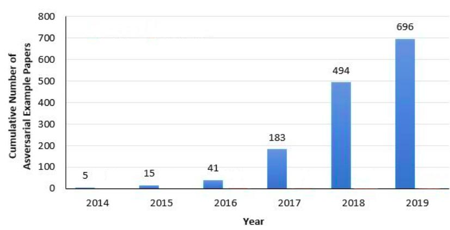
\includegraphics{Figures/figura_01.PNG}
\decoRule
\caption[Estudios publicados]{Estudios publicados asociados a seguridad en redes neuronales \parencite{r62}.}
\label{fig:estudios}
\end{figure}

El documento se compone de la siguiente forma, el capítulo \ref{Definiciones} presenta las definiciones necesarias para comprender el contenido del estudio, en él se explica de manera resumida el funcionamiento de las redes neuronales artificiales y sus tipos más comunes. El capítulo \ref{Ataques} presenta el estado del arte en cuanto a las técnicas de ataques a redes neuronales artificiales, luego el capítulo \ref{Defensa} expone las técnicas de defensas más conocidas. En el capítulo \ref{Experimentos} el lector podrá encontrar los experimentos realizados en el estudio en donde se realizan ataques a sistemas de visión artificial a través de la creación de ejemplos adversarios, utilizando distintas técnicas. También en este capítulo se brinda seguridad a un modelo de clasificación para hacerlo robusto frente a los ataques del experimento. Luego, en el capítulo \ref{Conclusiones} se exponen las conclusiones y resultados del estudio. Finalmente, en el capítulo \ref{Futuro} se presentan los lineamientos futuros sugeridos.


%----------------------------------------------------------------------------------------

\section{Objetivos}

Los objetivos de este estudio son los expuestos a continuación:
\begin{itemize}
\item Presentar un estado del arte de la seguridad en redes neuronales artificiales, exponiendo las distintas técnicas de ataque que pueden ser ejecutadas en contra de este tipo de modelo y presentar investigaciones sobre los tipos de defensas conocidos para hacer frente a dichos ataques.
\item Ejecutar pruebas de ataques en modelos de clasificación propios y presentar resultados que comprueben los estudios analizados.
\item Ejecutar pruebas de ataques en modelos de clasificación importados que sean de uso amplio y conocido para luego presentar resultados que comprueben los estudios analizados.
\item Proponer e implementar una contramedida que permita reducir el impacto de alguno de los tipos de ataques presentados en el estado del arte.
\end{itemize}

%----------------------------------------------------------------------------------------
